\documentclass{article}

%Um mit Latex zu arbeiten braucht man zwei Dinge:
% https://miktex.org/download
% https://www.xm1math.net/texmaker/download.html

%Hilfreiche Links:
%Sonderzeichen in Latex einfügen: https://de.wikibooks.org/wiki/LaTeX-Kompendium:_Sonderzeichen

\usepackage{xcolor}
\usepackage{graphicx}
\usepackage{listings}
\usepackage{float}
\usepackage{url}
\usepackage{verbatim}
\usepackage{multirow}
\usepackage{comment}
\usepackage{mathtools}
\usepackage[section]{placeins}
\usepackage{amsmath}
\usepackage{ulem}
\usepackage{cancel}
\newcommand{\mbeq}{\overset{!}{=}}
\DeclarePairedDelimiter\abs{\lvert}{\rvert}%

\title{Revision of "Measuring the beam profile"}
\author{Corinna Wegner, Garen Gregorian}

\begin{document}
\maketitle
\section{Abstract} 
%Wenn ich \subsection* schreibe (mit *), kommt diese Überschrift nicht in die Gliederung
In the original document, the resulting fit had many issues such as unphysical waist results and very uncharacteristic fit shapes. To correct, we added several measures to ensure a more accurate fit. Since we already know what to expect from the shape of the intensity function, we added the boundary condition (the power cannot be negative) in the fit that ensure the characteristic plateaus at the minimum and maximum intensities. Due to undersampling, these plateaus would not be accurately modeled otherwise. To further improve our model, the normalized micrometer positions were centered at zero to properly capture the expected (anti-)symmetry of the fit. Finally, bounds were also included to ensure that no negative values for waist could be calculated, as was a result without bounds since this would be an unphysical result.

\section{Measuring the beam profile}

In this experiment we measured the intensity of the laser light that is emitted by the fibre. We cut off some of the beam with a razor blade to see how much voltage is still measured by the photodiode. Thereby we obtained a profile of the beam cross section. After that we put a lens ($f=100mm$) behind the fibre end so that the beam was focused at the focal point. We measured the profile of the beam at different positions between the two lenses (the second lens ($f=50mm$) focuses the beam into the photodiode). Near the focal point of the first lens, where the waist of the gaussian beam lies, we measured three times. To eliminate fluctuations, we normalized the voltage signal with the other photodiode.\\

The total power the photodiode is detecting depends on the position of the razor blade $x$ and is given by:
\begin{equation}
P(x) = \int_x^\infty\mathrm{d}x' I_0 \mathrm{e}^{-\frac{2(x'-x_0)^2}{\omega^2}}.
\label{powerintegral}
\end{equation}

%\textcolor{red}{Beantworten: Welches Brechungsindexprofil müßte eine Glasfaser aufweisen, damit die Faser eine ideale Gauß-Mode führt?}

\paragraph{Measuring the cross section profile without focusing the beam}

To calculate the beam radius $\omega (z)$ we fitted the data of our measurement a (see appendix) to eq. \ref{powerintegral}. In order to do this we calculated the power from the voltage using:
\begin{equation}
P = \frac{hcU}{\lambda Re \eta}
\label{powerfromvoltage}
\end{equation} \\

The output parameters of the fit are:

$8,3cm:
 I_0: 0.008777106036129446 Strahltaille: 0.8825862418640391
11cm:
 I_0: 0.007991921587422922 Strahltaille: 1.0121807477924682
5,0cm:
 I_0: 0.010111526698723994 Strahltaille: 0.7755253848409015
waist: ( 0.8290558133524704 +- 0.053530428511568806 ) mm
rayleigh length: ( 3.4265554046505233 +- 0.4406541724660673 ) mm$

\begin{tabular}{ccc}
\hline
Label & $I_{0}$ (mW)& waist (mm) \\ 
\hline
$8.3cm$ & $8.777106036129446$ & $0.8825862418640391$\\ 
\hline
$11.0 cm$ & $7.991921587422922$ & $1.0121807477924682$\\ 
\hline
$5.0cm$ & $10.111526698723994$ & $0.7755253848409015$\\
\hline
%\label{part_a_results}
\end{tabular}

\textcolor{red}{Überarbeiten, neu interpretieren}
\textcolor{red}{Neue Werte eingeben}
The average waist is then $(\pm ) mm$. From that we also calculated the rayleigh length 
\begin{equation}
z_{R} = \frac{\pi\omega_{0}^2 n}{\lambda} 
\label{rayleighlength}
\end{equation}
at which the beam radius is $\sqrt{2}\omega_{0}$. In our case, $n=1$ is the refraction index of the medium (air) and the wavelength of the laser is $\lambda =632.8 nm$. The resulting rayleigh length is:
$(3.4 \pm 0.4) mm$.\\

\begin{figure}
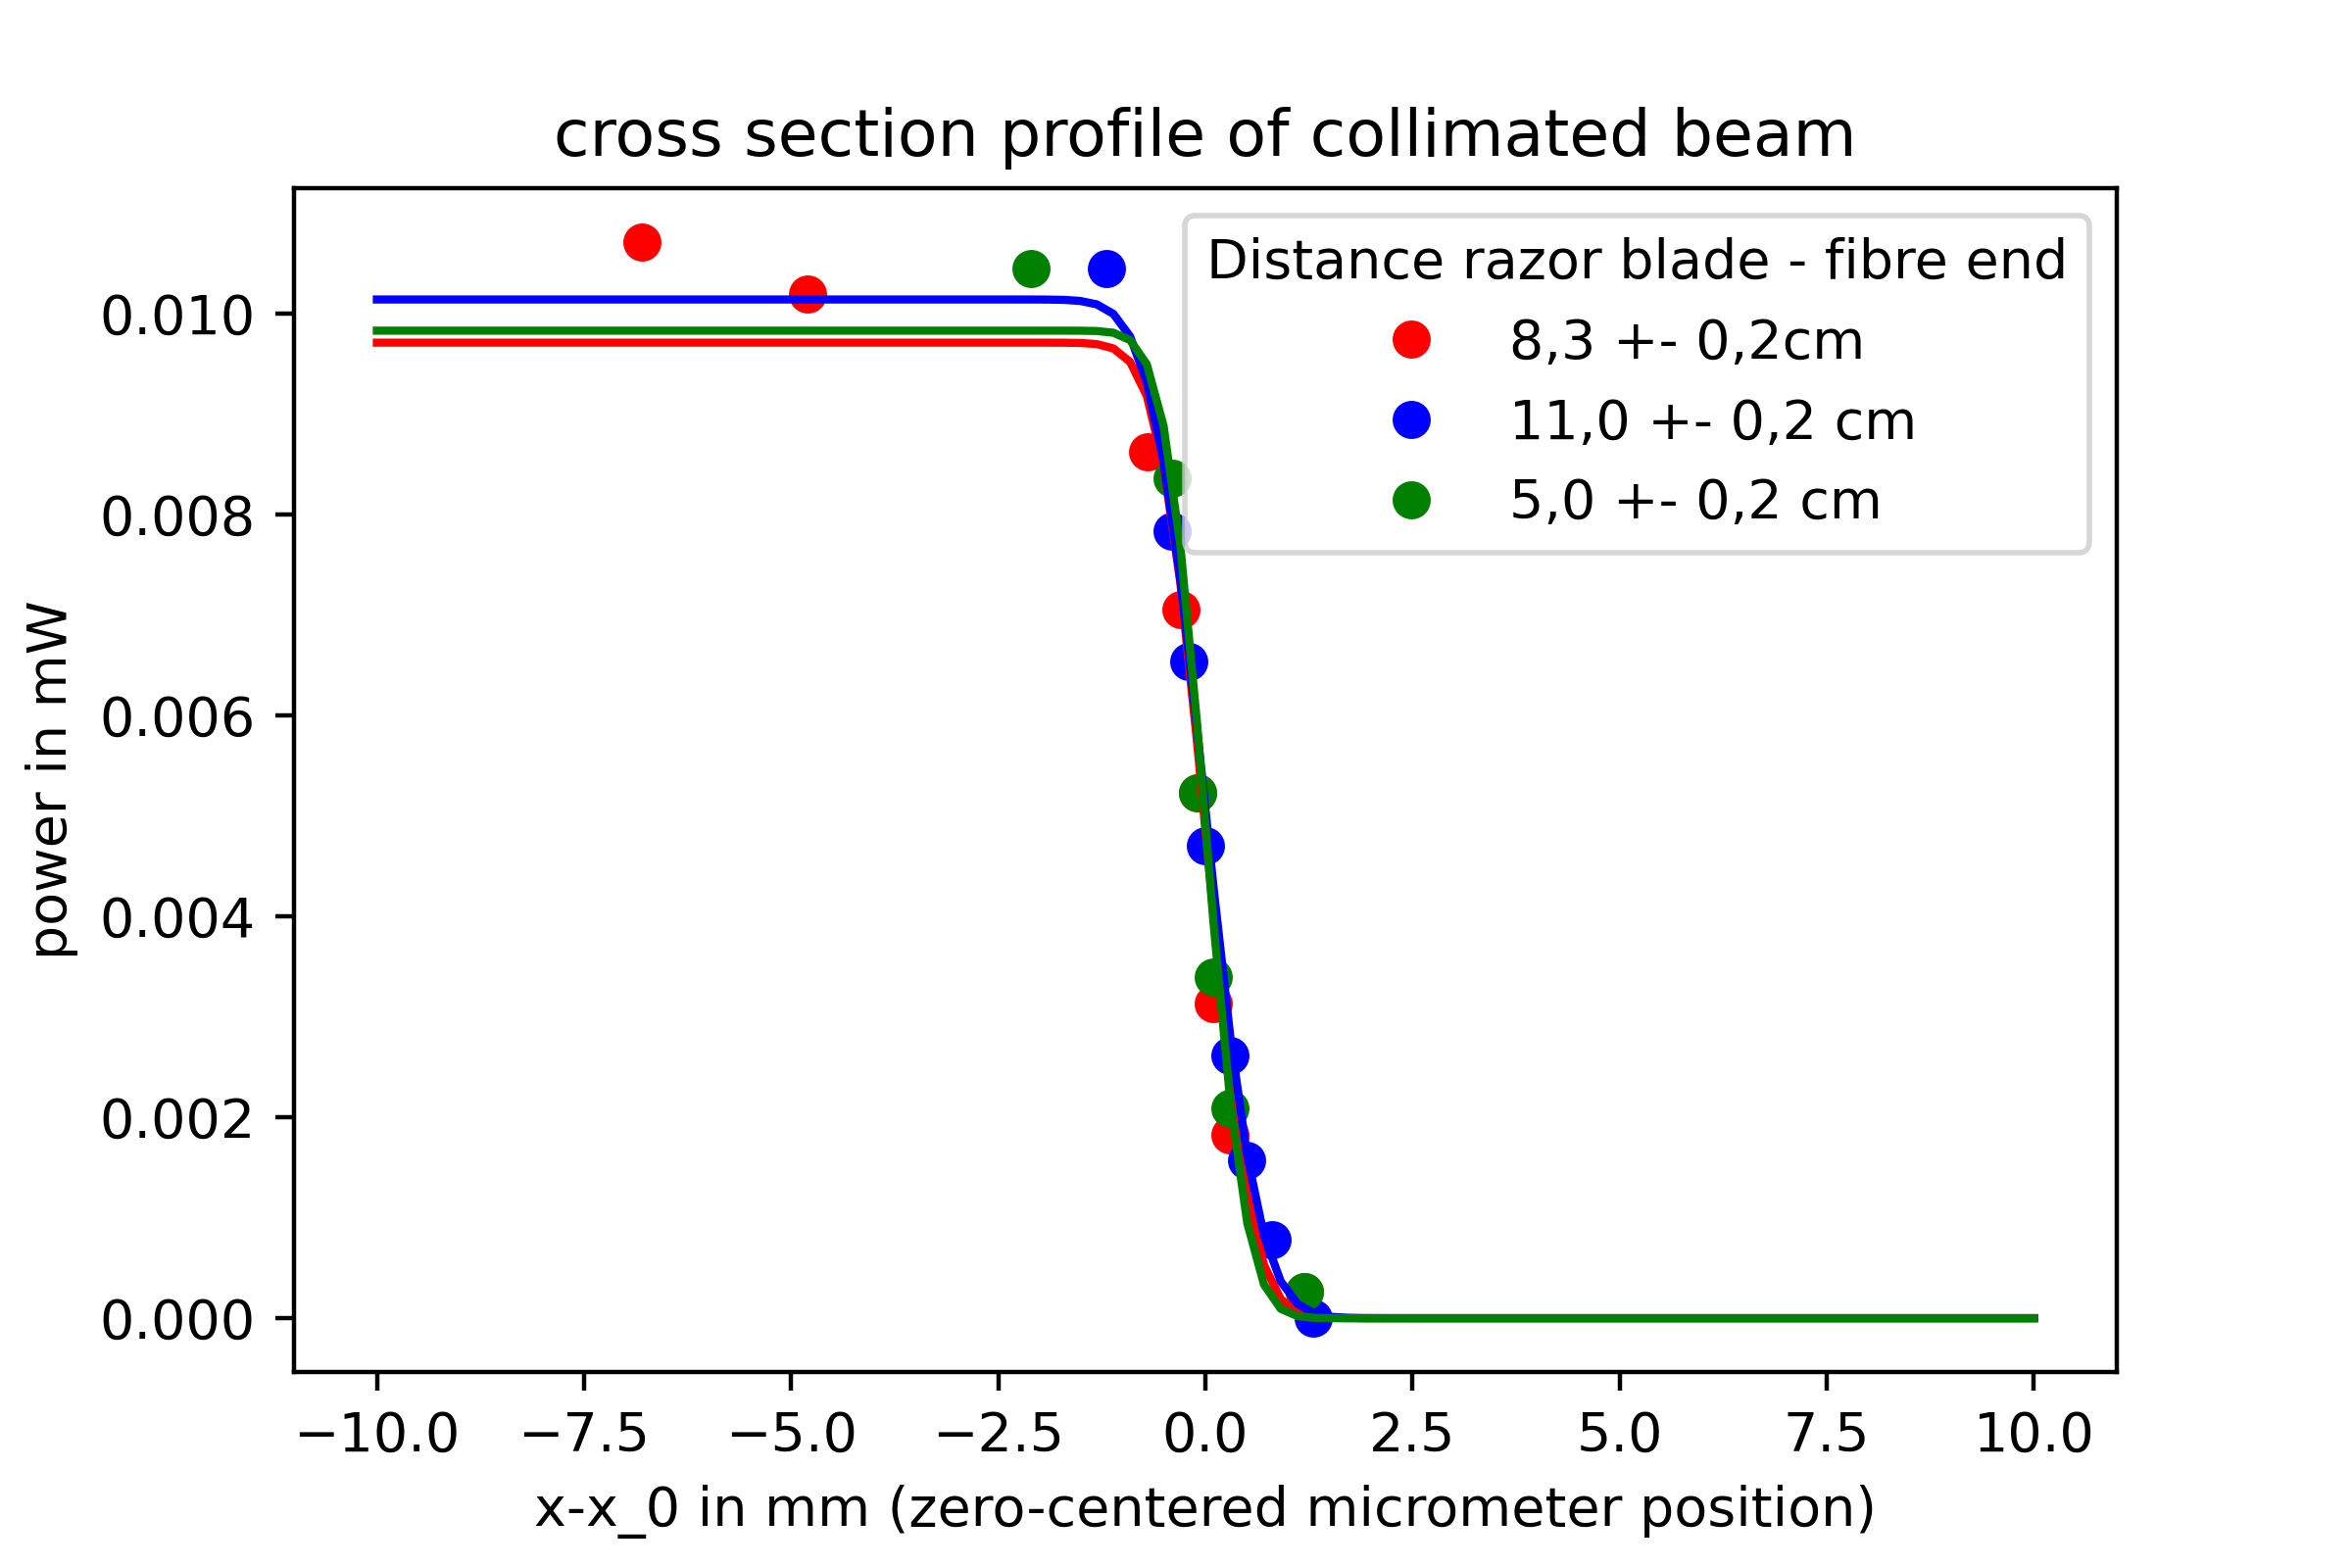
\includegraphics[width=\textwidth]{cross section profile of collimated beam.png}
\caption{cross section profile of collimated beam}
\label{part_a_fig} %Man kann mit \ref{part_a_fig} auf dieses Bild verweisen
\end{figure}

\textcolor{red}{Überarbeiten}
The first two measurements of the series with Distance razor blade - fibre end $= 8.3 cm$ seemed to fall out of line. When doing the fit, the curve (red dashed) also looked inappropiate. Presumably we measured these points too early, namely not at the point right before the power falls off (i.e. the maximum). Therefore we decided to leave them out of the fitting, which lead to a much better result (see figure \ref{part_a_fig}).

The relatively high errors can be explained by the strong fluctuations of the multimeter display, making it hard to measure the voltage. This can be seen when looking at the next figure, where the measurement points differ quite a lot from the fit curves. However, one can see that the shapes of the fit curves look similar. Another problem of the experiment was that there could be scattering light from the ambient or laser, which influences the photodiode. Furthermore the razor did not really fit the radial intensity profile of the beam. It only cuts off the beam from one direction, leaving the other direction always open. Therefore there is a systematic error in the experiment. Using an apperture would have been a better way to measure the beam profile. Also, in order to measure at certain distances from the fibre end, we had to put the razor mount into a place between the threads where you can fix the mount on the table. This could lead to a non orthogonal angle between razor and beam, which would mean that you have to turn the micrometer screw more to get the same decrease of intensity. Besides, at the edge of the razor there is diffraction happening, as we have examined in a previous practical. This could also skew the measurements. Finally it was hard to measure the distances in the $z$-direction having only a ruler. The experiment was very barred by the coupler and other optical instruments, so a caliper would have helped to increase the quality of those measurements.

\paragraph{Measuring the cross section profile with lens ($f=100mm$)}

We measured the beam profile using the razor blade technique at seven distances from the lens. Three measurements were taken near the focal point because here we expected the waist $\omega_{0}$, i.e. the minimum of the beam radius $\omega (z)$. They are related by the equation:
\begin{equation}
\omega (z) = \omega_{0}\sqrt{1+\frac{z^2}{z_{R}^2}}
\label{omegaofz}
\end{equation}

The razorblade positions z from which we measured the beam profile are $-(7.0\pm 0.2)cm, -(4.0\pm 0.2)cm, -(1.0\pm 0.2)cm, (0.0\pm 0.2)cm, (1.0\pm 0.2)cm, (4.3\pm 0.2) cm$ and $(7.0\pm 0.2)cm$, where $z=0$ is the focal point. For illustration purposes we plotted the data near focal point in an extra plot. The plots show the calculated powers (equation \ref{powerfromvoltage}) from the measuring data along with the corresponding fit to the gaussian integral (equation \ref{powerintegral}). From the fit we obtained $I_{0}$ and $\omega(z)$:

$Rot: I_0: 0.0314677004624013 Strahltaille: 0.21386318820116362
Blau: I_0: 0.07270445083092966 Strahltaille: 0.0774080737868041
Grun: I_0: 0.029874937606379274 Strahltaille: 0.15819545705252225
Gelb: I_0: 0.015763387087890192 Strahltaille: 0.37413622790241946
turkis: I_0: 0.06136075469487003 Strahltaille: 0.08303635608624456
magenta: I_0: 0.06379644469561196 Strahltaille: 0.08349636759598762
schwarz: I_0: 0.004440113074039632 Strahltaille: 1.549232366989364$

\begin{tabular}{ccc} 
  \hline
  Label & $I_{0}$ (W)& waist (mm) \\ 
  \hline
  $-7.0 cm$ &$0.06136075469487003 $ & $0.08303635608624456 $\\ 
  \hline
  $-4.0 cm$ &$0.015763387087890192 $ &$ 0.37413622790241946$\\ 
  \hline
  $-1.0cm$ &$0.07270445083092966 $ &$0.0774080737868041$\\
  \hline
  $0.0 cm$ &$0.0314677004624013 $ &$ 0.21386318820116362 $\\ 
  \hline
  $1.0 cm$ &$0.029874937606379274 $ &$0.15819545705252225 $ \\
  \hline
  $4.3 cm$ &$0.06379644469561196 $ & $ 0.08349636759598762$ \\ 
  \hline
  $7.0 cm$ & $ 0.004440113074039632$ & $1.549232366989364 $\\
  \hline 
%\label{part_b_results}
\end{tabular}

\textcolor{red}{Überarbeiten, interpretieren, warum ein Wert extrem...}

Again, we fitted the measurement series for each razor-lens-distance $z$ to eq. \ref{powerintegral} and obtained the local $\omega(z)$. Then we fitted these together with the corresponding $z$ to eq. \ref{omegaofz}.
From that we obtained the waist\\ 
$\omega_{0} = ( 1 \pm 6 ) mm $\\
The resulting rayleigh length is\\
$z_{R} =  ( 1 \pm 7 ) mm $\\

\textcolor{red}{y-Achsenbeschriftung noch von W in mW ändern oder so ähnlich}

\begin{figure}[h!]
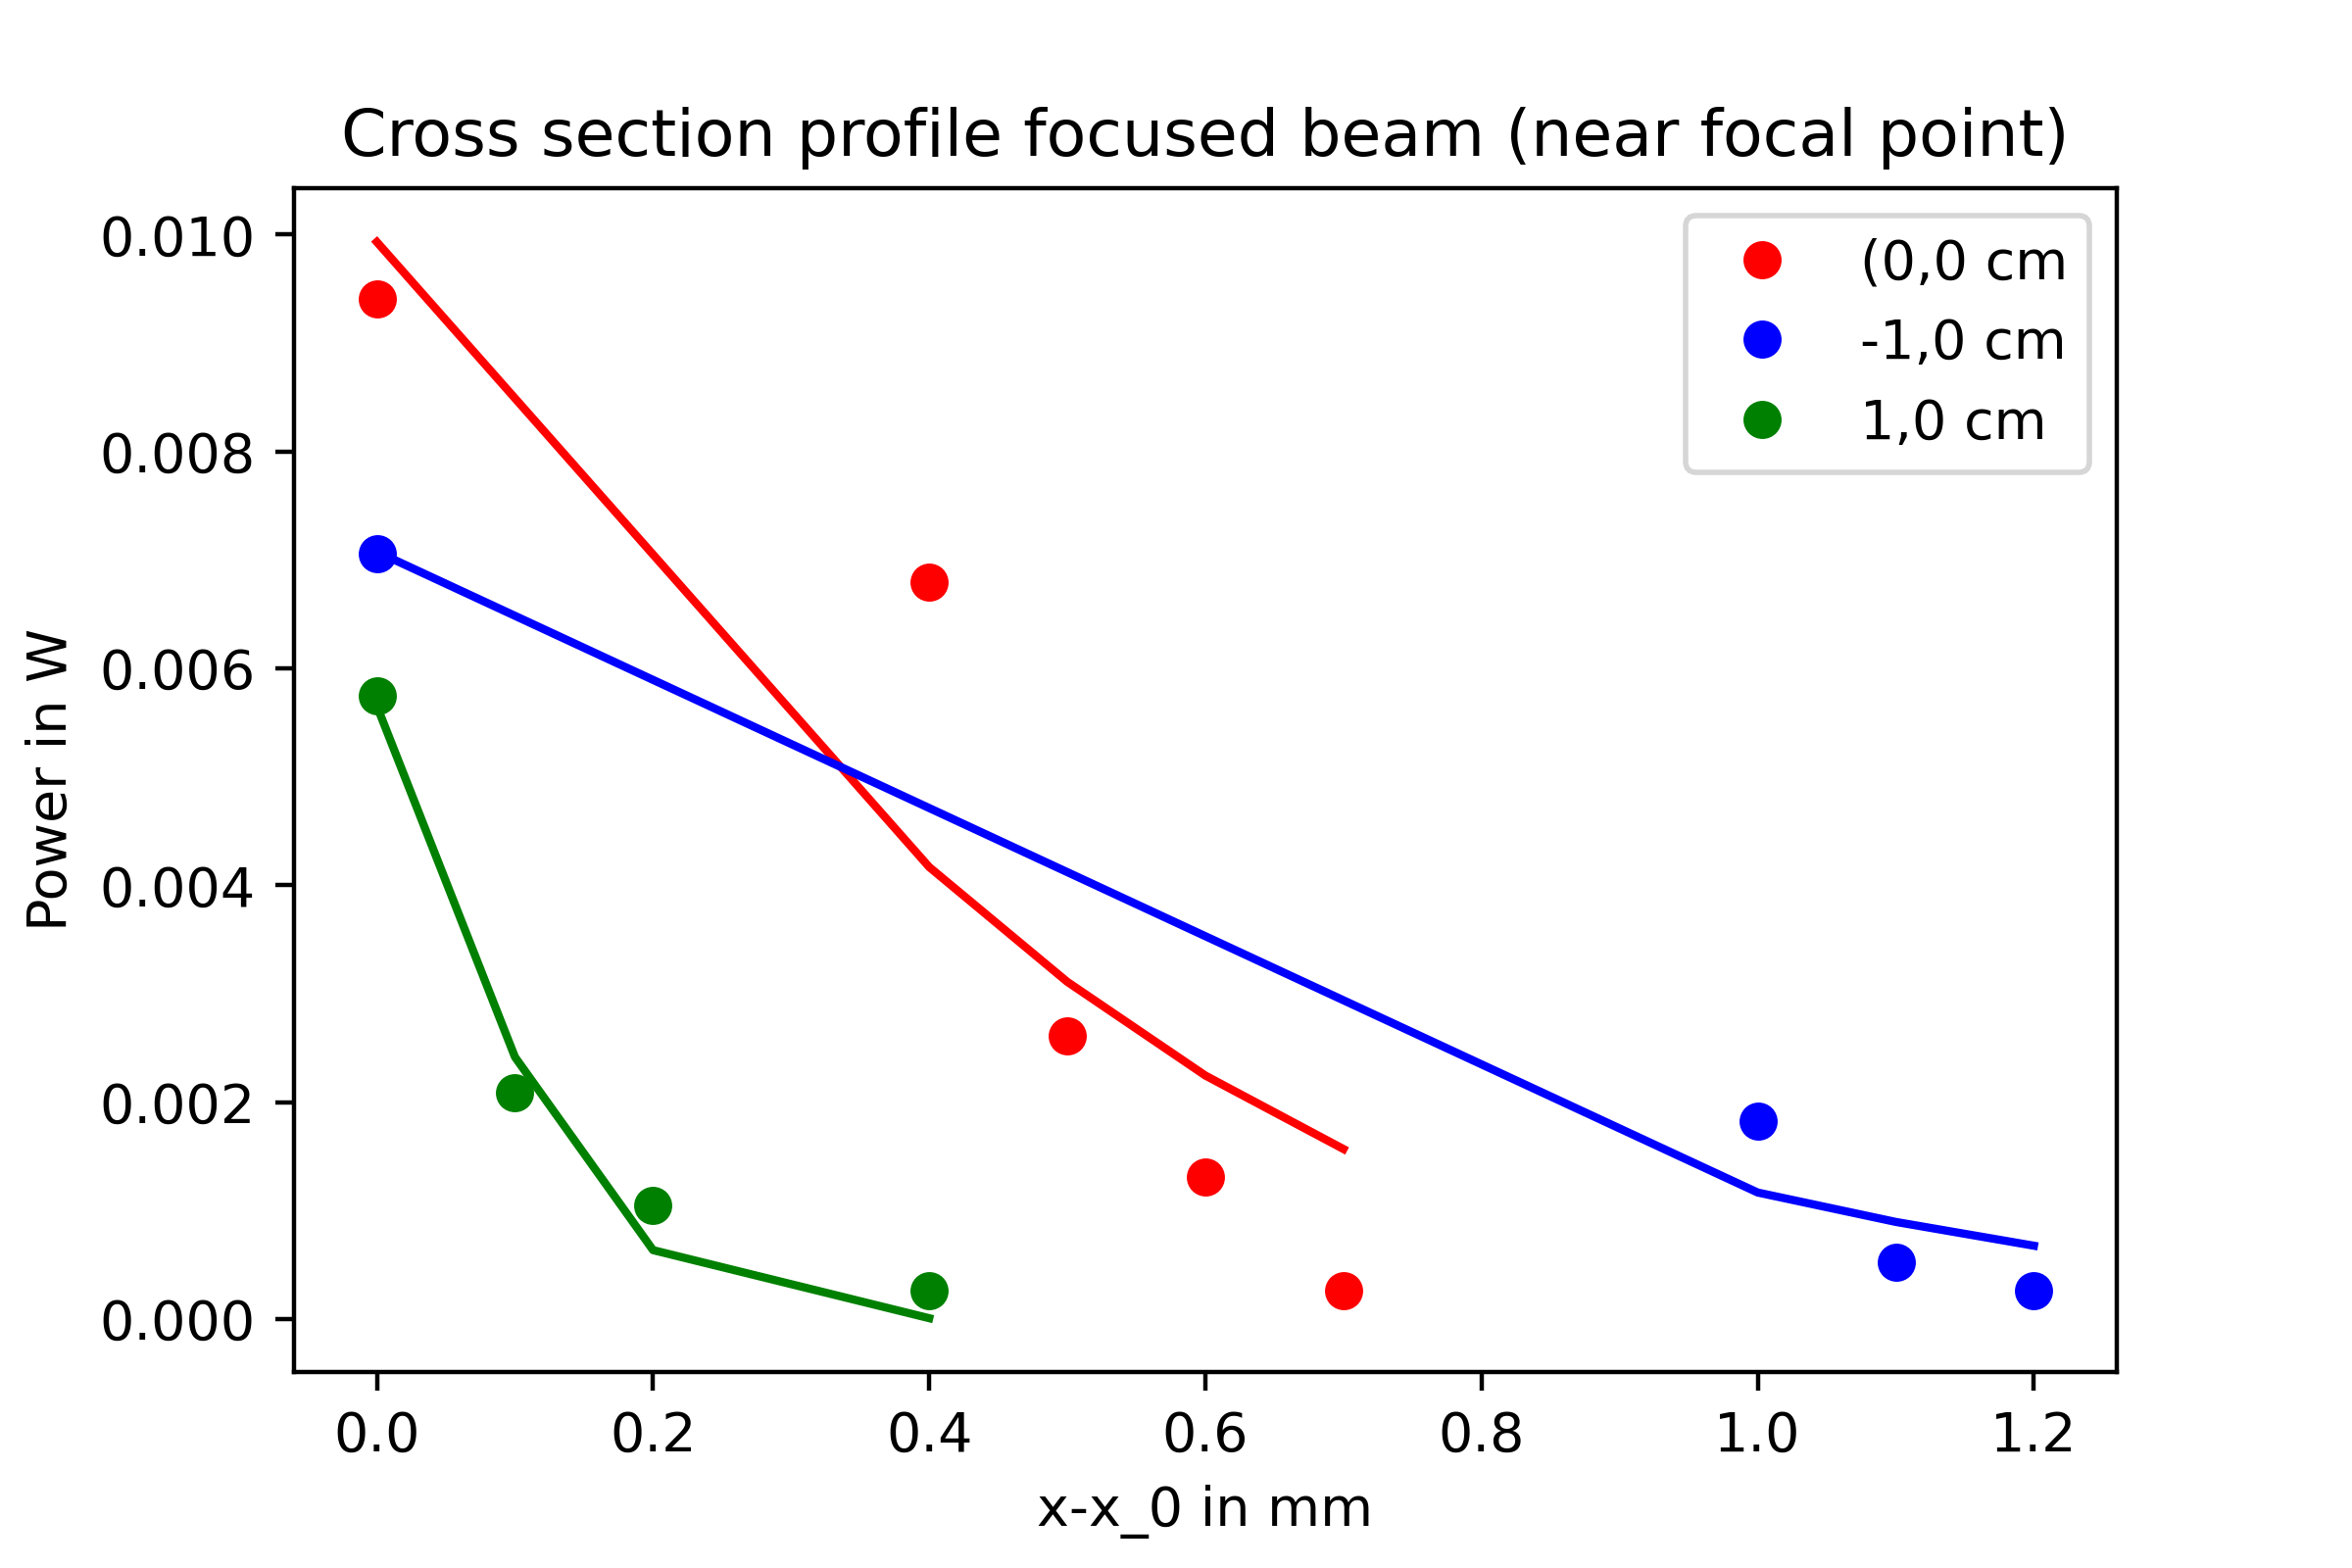
\includegraphics[width=\textwidth]{Cross section profile focused beam (near focal point).png} 
\caption{Cross section profile focused beam (near focal point)}
\label{near_focal} 
\end{figure}

\begin{figure}[h!]
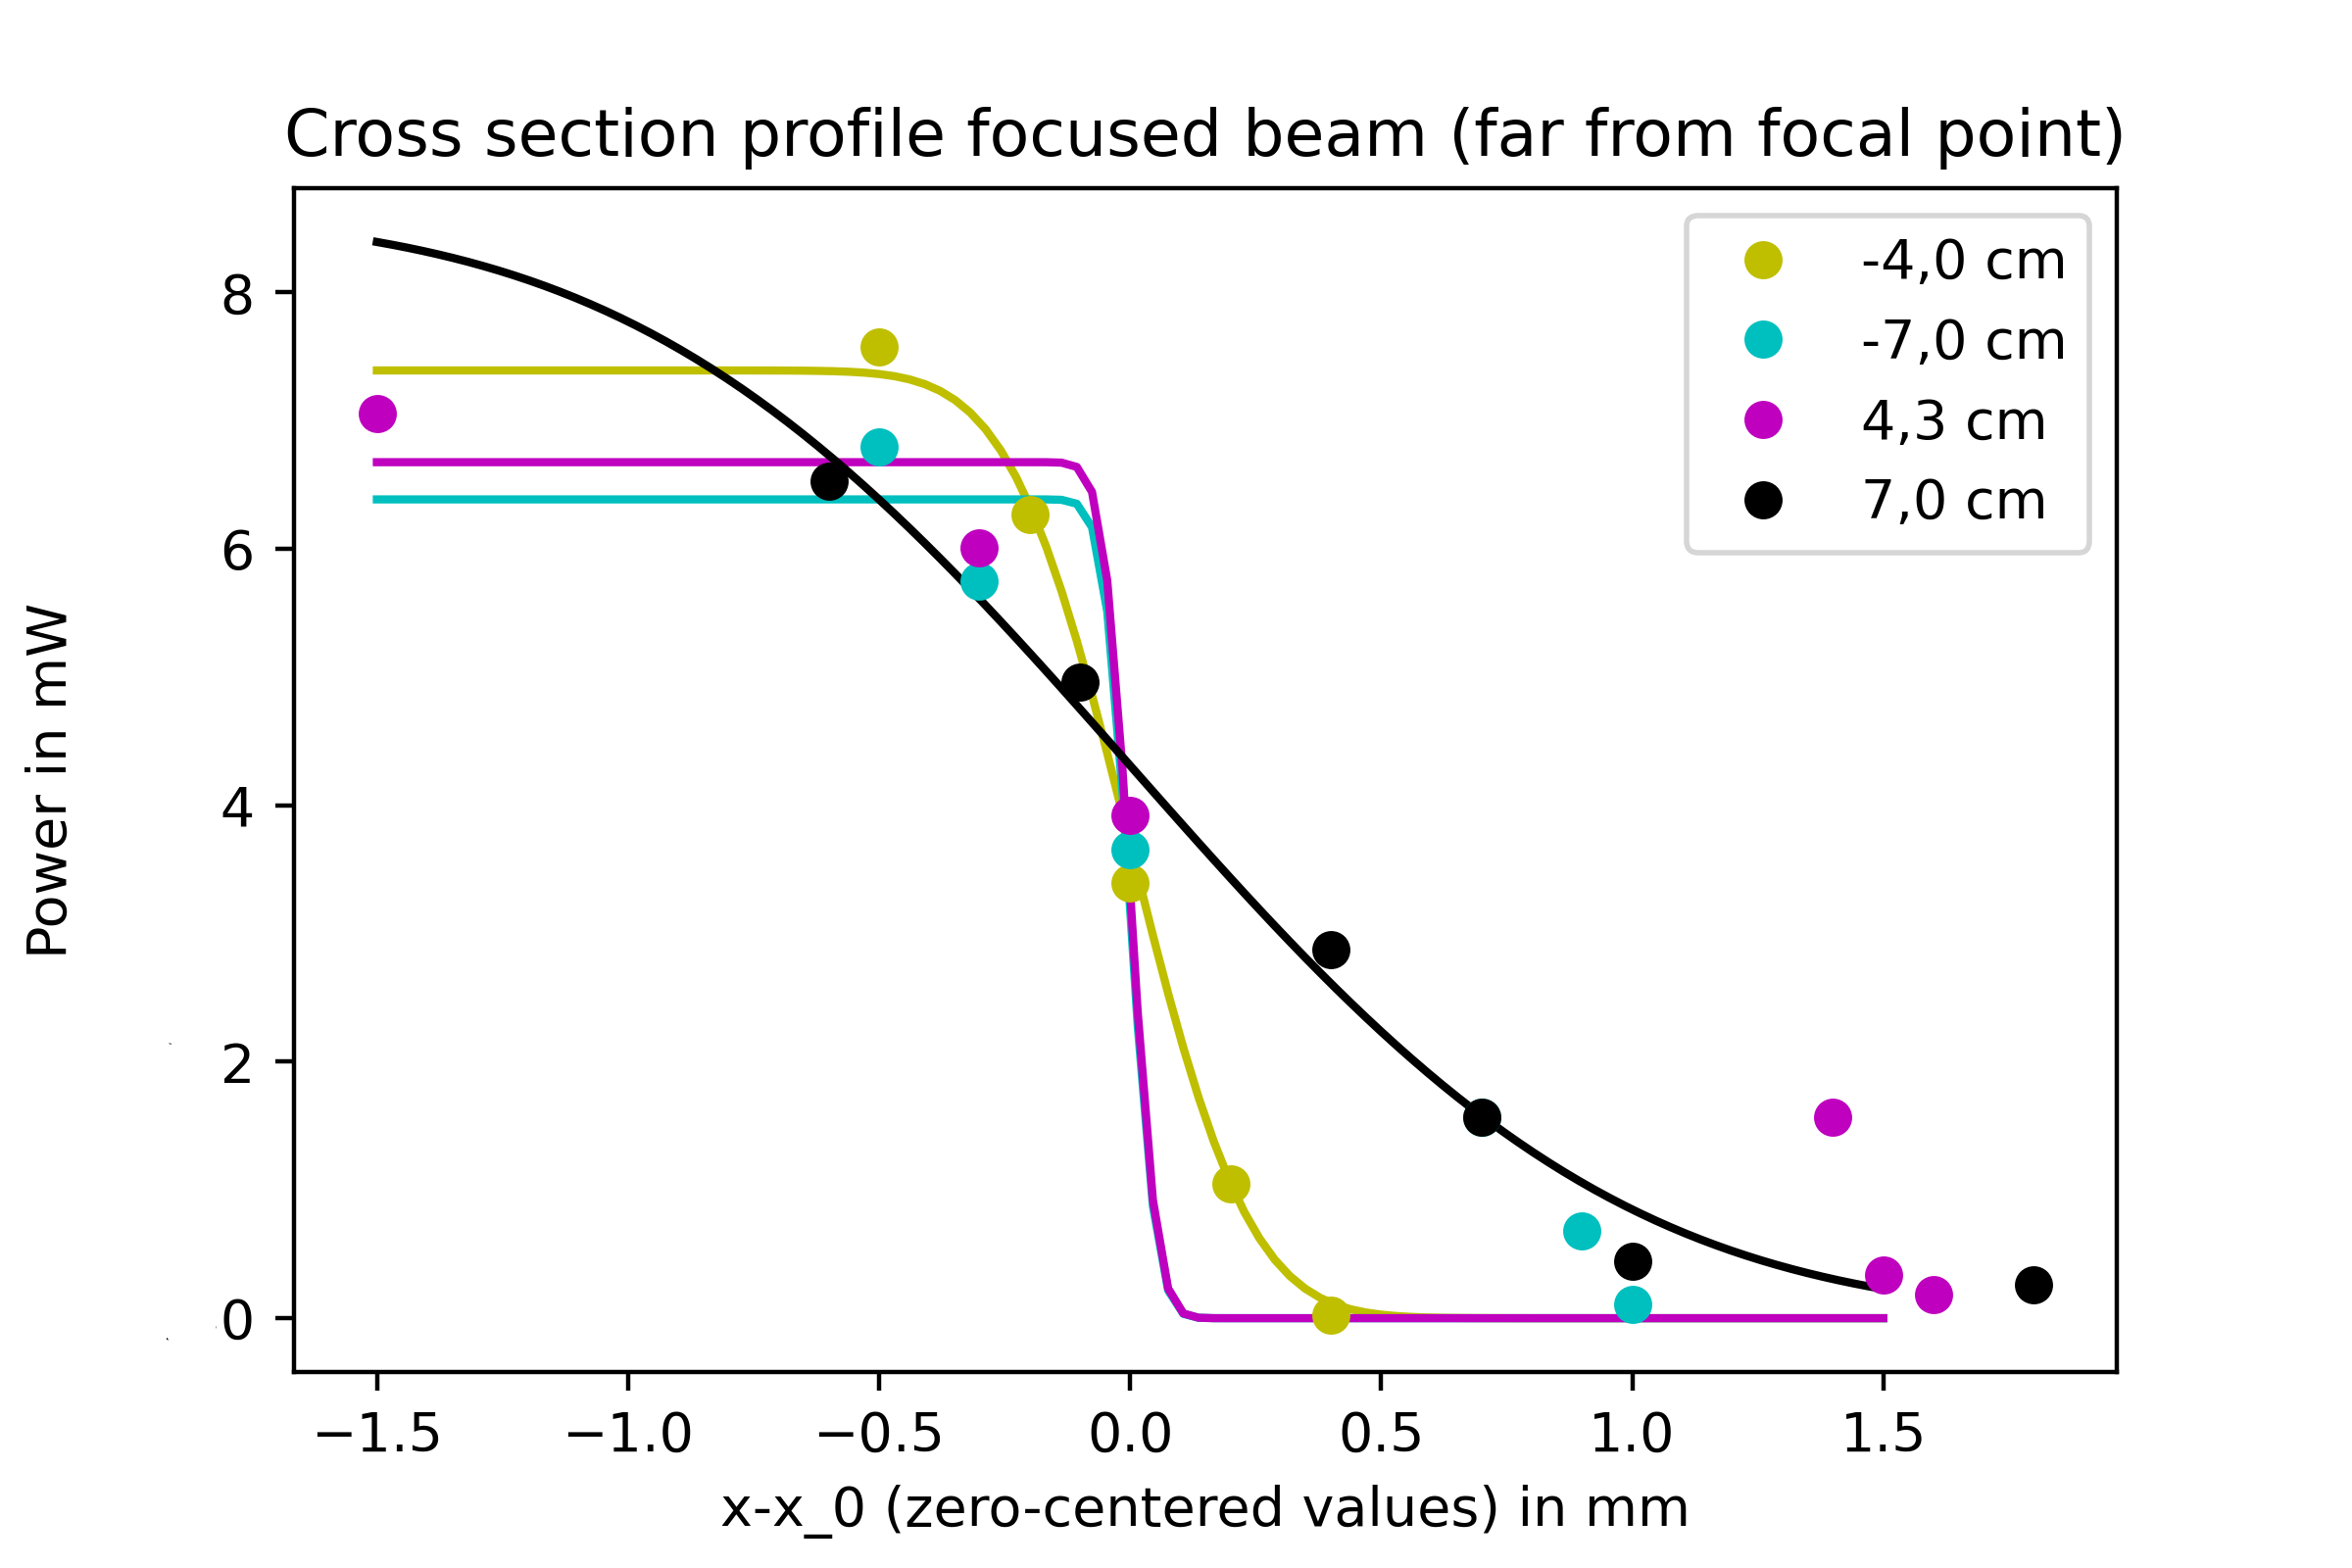
\includegraphics[width=\textwidth]{Cross section profile focused beam (far from focal point).png}
\caption{Cross section profile focused beam (far from focal point)}
\label{far_focal}
\end{figure}

\begin{figure}[h!]
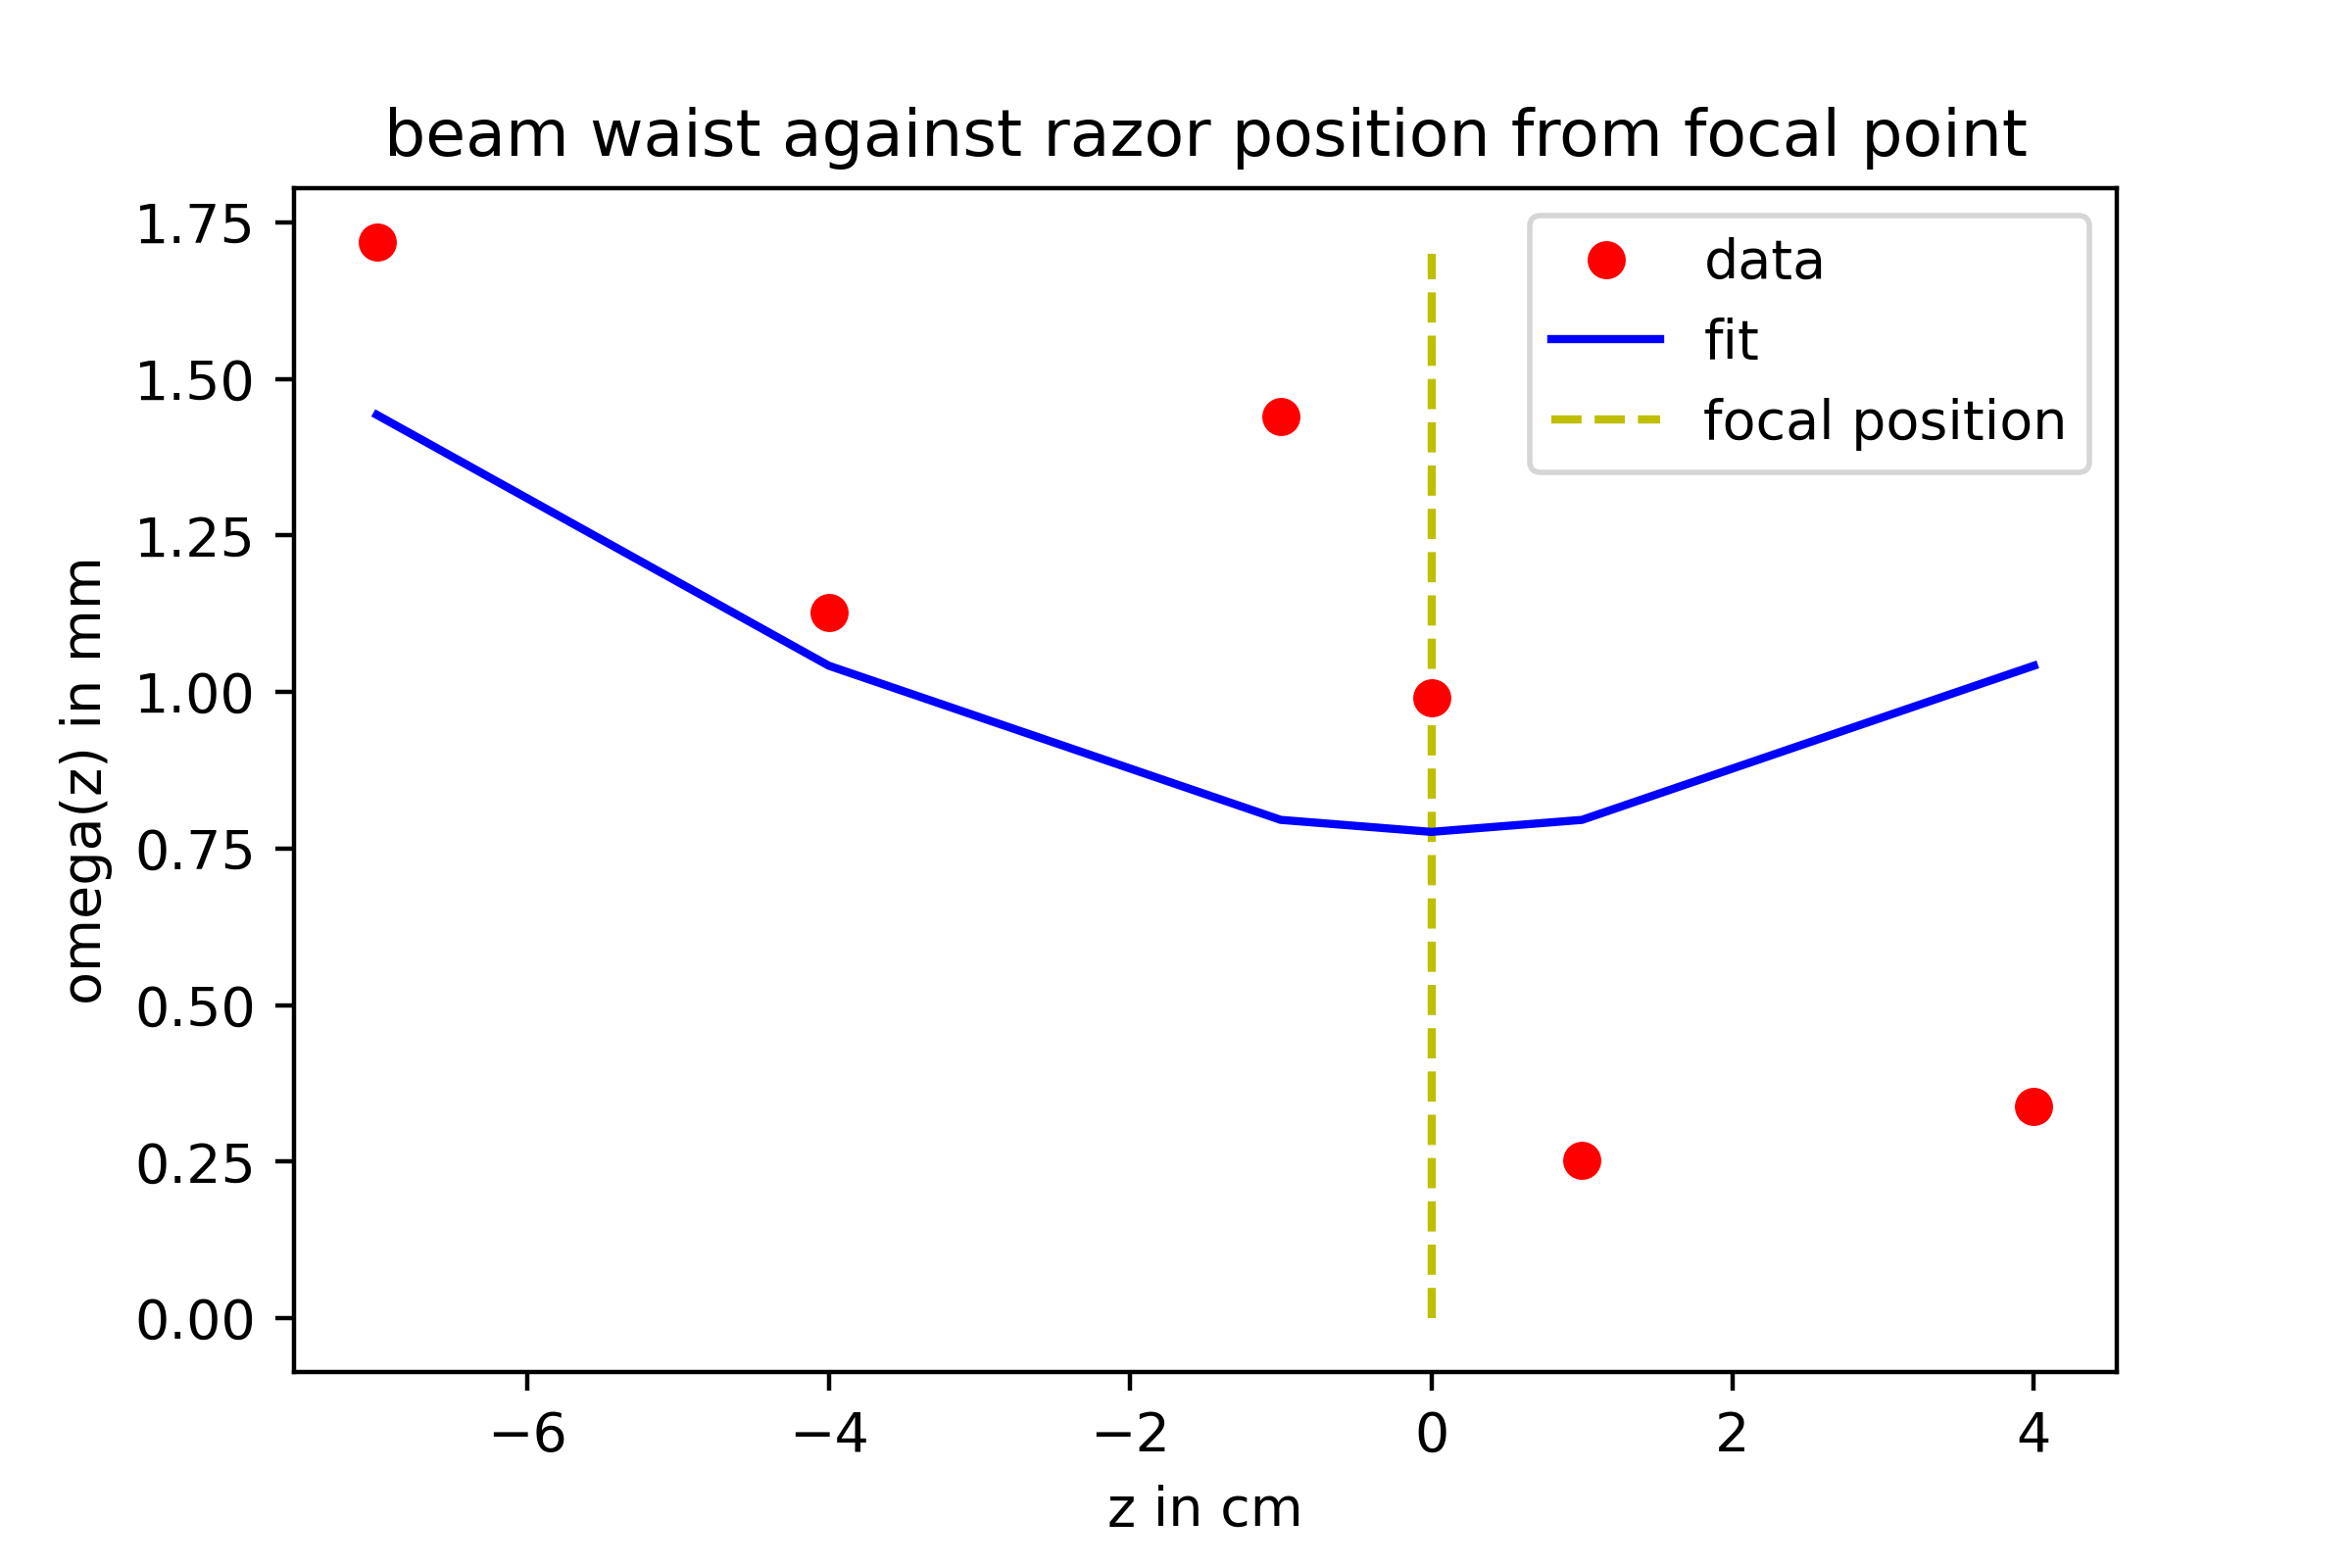
\includegraphics[width=\textwidth]{beam waist against razor position from focal point.png}
\caption{Beam waist against razor position from focal point}
\label{beam_waist}
\end{figure}

\textcolor{red}{Überarbeiten}
As in the previous part, we see that the standard deviations of $\omega_{0}$ and $z_{R}$ are relatively high. This time for the rayleigh length is is even higher than the value itself, which is illogical because it includes negative values within the error range. Since the experiments are very similar, the discussed error sources apply as well here. Furthermore, we observed extreme fluctuations on the multimeter display especially when measuring near the focal point. A reason for this could be that the waist is so small such that even the tiniest micrometer screw turn makes a lot of difference. In fact, sometimes only contact with the table changed the displayed value by about 20 mV. To avoid abberations we made sure the beam enters the plano-convex lens on its curved surface, such that the refraction takes place on both surfaces of the lens. Nevertheless we could only approximately determine the center of the lens and thereby abberations can not be excluded totally.

\section{Appendix}

\lstset{literate=
  {á}{{\'a}}1 {é}{{\'e}}1 {í}{{\'i}}1 {ó}{{\'o}}1 {ú}{{\'u}}1
  {Á}{{\'A}}1 {É}{{\'E}}1 {Í}{{\'I}}1 {Ó}{{\'O}}1 {Ú}{{\'U}}1
  {à}{{\`a}}1 {è}{{\`e}}1 {ì}{{\`i}}1 {ò}{{\`o}}1 {ù}{{\`u}}1
  {À}{{\`A}}1 {È}{{\'E}}1 {Ì}{{\`I}}1 {Ò}{{\`O}}1 {Ù}{{\`U}}1
  {ä}{{\"a}}1 {ë}{{\"e}}1 {ï}{{\"i}}1 {ö}{{\"o}}1 {ü}{{\"u}}1
  {Ä}{{\"A}}1 {Ë}{{\"E}}1 {Ï}{{\"I}}1 {Ö}{{\"O}}1 {Ü}{{\"U}}1
  {â}{{\^a}}1 {ê}{{\^e}}1 {î}{{\^i}}1 {ô}{{\^o}}1 {û}{{\^u}}1
  {Â}{{\^A}}1 {Ê}{{\^E}}1 {Î}{{\^I}}1 {Ô}{{\^O}}1 {Û}{{\^U}}1
  {ã}{{\~a}}1 {ẽ}{{\~e}}1 {ĩ}{{\~i}}1 {õ}{{\~o}}1 {ũ}{{\~u}}1
  {Ã}{{\~A}}1 {Ẽ}{{\~E}}1 {Ĩ}{{\~I}}1 {Õ}{{\~O}}1 {Ũ}{{\~U}}1
  {œ}{{\oe}}1 {Œ}{{\OE}}1 {æ}{{\ae}}1 {Æ}{{\AE}}1 {ß}{{\ss}}1
  {ű}{{\H{u}}}1 {Ű}{{\H{U}}}1 {ő}{{\H{o}}}1 {Ő}{{\H{O}}}1
  {ç}{{\c c}}1 {Ç}{{\c C}}1 {ø}{{\o}}1 {å}{{\r a}}1 {Å}{{\r A}}1
  {€}{{\euro}}1 {£}{{\pounds}}1 {«}{{\guillemotleft}}1
  {»}{{\guillemotright}}1 {ñ}{{\~n}}1 {Ñ}{{\~N}}1 {¿}{{?`}}1 {¡}{{!`}}1 
}

\textcolor{blue}{Measuring the beam profile (a)}\\
\lstinputlisting[language=python]{Strahlprofil_a.py}
\textcolor{blue}{Measuring the beam profile (b)}\\
\lstinputlisting[language=python]{Strahlprofil_b_v2.py}

\end{document}